\glsresetall
The \gls{qmla} framework lends itself easily to the family of optimsation techniques called \emph{evolutionary algorithms}, 
    where individuals, sampled from a population of candidates, are considered as solutions to the given problem.
Candidates are batched in \emph{generations},
    such that iterative generations aim to efficiently search the available population
    by mimicing biological evolutionary mechanisms \cite{back1996evolutionary}. 
In particular, we develop an \gls{es} which incorporates a \gls{ga} in the construction of models;
    \glspl{ga} are a subset of evolutionary algorithms where candidate solutions are expressed as 
    strings of numbers representing some configuration of the system of interest \cite{holland1992adaptation}.
We describe the concepts of \glspl{ga} in \cref{sec:genetic_algorithms}, 
    so we begin this chapter by describing the adaptations which allow us to build a \gls{ges} within \gls{qmla}. 
\par 

\section{Adaptation to QMLA framework}\label{sec:ga_adaptation_to_qmla}
Unlike the generic aspects of \glspl{ga} described in \cref{sec:genetic_algorithms}, 
    in the context of \gls{qmla}, we must deviate from default mechanisms. 
The overarching goal of \gls{qmla} --
    to characterise some black box quantum system, \gls{q} --
    proceeds by designing and performing experiments upon \gls{q} which enable us to improve 
    the modelling of $\ho$. 
Nothing described so far provides a natural \gls{of}, upon which \glspl{ga} rely 
    to assess the suitability of candidates relative to contemporaries.
We can not assume knowledge of $\ho$ while generating candidates \glspl{model},
    so we can not simply invoke some loss function with respect to the target model, for example. 
Instead, we must devise schemes which exploit the knowledge we \emph{do} have about each candidate $\hj$, 
    which is the primary challenge in building an \gls{es} based on a \gls{ga}.  
We propose and discuss a number of options in \cref{sec:objective_functions}. 
\par 

Common to all proposed \glspl{of}, however, is that candidates should first be trained before evaluation, 
    so that their assessment is based on their actual power in describing \gls{q},  
    rather than some initial paramterisation which may not capture their potential. 
This is a tenet of \gls{qmla}: for each candidate $\hj ( \al_j )$, we use a subroutine to optimise $\al_j$;
    as in earlier applications of \gls{qmla}, for this study we rely on \gls{qhl} as the parameter optimisation subroutine. 
\par

Ultimately, the conceived role of a \gls{ga} within \gls{qmla} is to generate the sets of models to place 
    on successive branches\footnote{Branches in \gls{qmla} and generations of the \glsentrylong{ga} are equivalent here.} 
    of an \gls{et} as depicted in \cref{fig:qmla_overview}.
The apparatus within \gls{qmla} which facilitates novel model generation techniques is the \glsentryfull{es}.
Here we will design an \gls{es} which acts in cooperation with a \gls{ga}:
    the \gls{es} specifies that consolidation of a generation $\mu$ involve evaluating the \emph{fitness}, 
    $g_i$, of each candidate, $\hi$, via the chosen \gls{of}; 
    the \gls{ga} then maps $\{g_i\}$ of each $\hi \in \mu$ to a selection probability, 
    and composes new candidates via crossover, \cref{sec:reproduction}. 
Recall from \cref{sec:model_generation}, that we capture the space of available terms as $\termset$, 
    i.e. we list -- in advance -- the feasible terms which may be included in candidate models\footnotemark, 
    with $N_t = | \termset |$ the number of terms considered. 
\gls{qmla} is then an optimisation algorithm, attempting to find the set $\termset^{\prime}$
    which \emph{best} represents the true terms $\termset_0$.
Note, this does not require idenitifcation of the precise \gls{true model} to be successful, 
    as insight can be gained from approximate models which capture the physics of the target system. 
We introduce metrics for success in \cref{sec:f_score}. 
We recognise the limitations this structure imposes: we can only identify terms which were conceived in advance; 
    this may restrict \gls{qmla}'s applicability to entirely unknown systems, 
    where such a primitive set can not even be compiled.  
\footnotetext{
    Recall that models impose structure on sets of terms: $\hj = \al_j \cdot \vec{T}_j = \sum_{k \in \{j\}} \alpha_k \hat{t}_k$.
}    
\par 

The structure of the overall \gls{qmla} algorithm (recall \cref{fig:qmla_overview}) is unchanged.
In a \gls{ges}:
\begin{easylist}[itemize]
    & Branches: models are still grouped in branches, here called generations;
    & Training: models are still trained, again through \gls{qhl};
    & Consolidation: all models are evaluated according to the \gls{of} to be described in \cref{sec:objective_functions}, 
        so branches are consolidated by ranking models according to their fitness;
    & Spawning: new models are spawned through the \gls{ga} by selecting pairs of parents for crossover, 
        with the resultant offspring models probabilistically mutated. 
\end{easylist}
\par 

The design of any \gls{es} centres on the implementation of the 
    \ttt{generate\_models} subroutine -- we summarise the \gls{ges}'s method in \cref{alg:ga_generate_models}. 
We can restate the informal description of \glspl{ga}\footnotemark, now in the context of \gls{qmla}, as
\footnotetext{First stated on \cpageref{mark:informal_ga}.}

\begin{easylist}[enumerate]
    \ListProperties(Numbers2=l, Numbers3=r)
    & Sample $N_m$ models from $\population$ at random
    && this is the first generation, $\mu$. 
    & \label{qmla_ga:loop} Evaluate each model $\hj \in \mu$
    && train $\hj$ through \gls{qhl};
    && apply the \glsentrylong{of} to assign the model's fitness, $g_j$.
    & Map the fitnesses of each model, $\{g_j\}$, to selection probabilities for each model, $\{s_j\}$
    && e.g. by normalising the fitnesses, or by removing some poorly-performing models and then normalising. 
    & Generate the next generation of models
    && Reset $\mu = \{ \}$;
    && \label{qmla_ga:select} Select pairs of parents, $\h_{p_1}, \h_{p_2}$, from $\mu$
    &&& Each model's probability of being chosen is proportional to their $s_j$;
    && Cross over $\h_{p_1}, \h_{p_2}$ to produce children models, $\h_{c_1}, \h_{c_2}$
    &&& mutate $\h_{c_1}, \h_{c_2}$ according to some random probabilistic process;
    &&& $\mu \gets \mu \cup \{\h_{c_i} \}$, only if $\h_{c_i}$  is not already in $\mu$, 
        to ensure $N_m$ unique models are tested at each generation;
    && until $| \mu| = N_m$, iterate to step (\ref{qmla_ga:select}.
    & Until the $N_g^{th}$ generation is reached, iterate to step \ref{qmla_ga:loop}.
    & The strongest model on the final generation is deemed the approximation to the system, $\hp$. 
\end{easylist}



\par 

\subsection{Models as chromosomes}
We first need a mapping from models to chromosomes; 
    this is straightforward given the description of chromosomes as binary strings, 
    exemplified in \cref{sec:knapsack}. 
We assign a gene to every term in $\termset$, so that candidate models are succinctly represented by bit strings of length $N_t$. 
We give an example of the mapping between models and chromosomes in \cref{table:chromosome_example}.
Given that every model is contained in the space of bit strings spanned by $N_t$ bits, 
    we can say that there are a total of $2^{N_t}$ available models in the \gls{model space}. 


\begin{table}

    \renewcommand{\arraystretch}{2.0}
    \setlength{\tabcolsep}{5pt}

    \def\rowbox#1#2{%
        \smash{\color{#2}\fboxrule=1pt\relax\fboxsep=2pt\relax%
        \llap{\rlap{\fbox{\vphantom{0}\makebox[#1]{}}}~}}\ignorespaces
    }

    \definecolor{parentA}{HTML}{002bd8} % blue
    \definecolor{parentB}{HTML}{316c00} % green
    \definecolor{mutation}{HTML}{961f29} % red
    \newcommand\parentcolourA{parentA}
    \newcommand\parentcolourB{parentB}
    \newcommand\mutationcolour{mutation}

    % \newcommand\parentcolourA{blue}
    % \newcommand\parentcolourB{green}
    % \newcommand\mutationcolour{red}

    \newcommand\longrowboxlenth{185pt}
    \newcommand\shortrowboxlength{80pt}
    
    \begin{center}
    \begin{tabular}{ c  c | c  c  c  c  c  c } 
            \hline
        \multicolumn{2}{c|}{Model} & \multicolumn{6}{c}{Chromosome} \\
        & $\terms$ & $\hat{\sigma}_{(1,2)}^{x}$ & $\hat{\sigma}_{(1,2)}^{z}$ & $\hat{\sigma}_{(2,3)}^{y}$ 
            & $\hat{\sigma}_{(2,3)}^{x}$ & $\hat{\sigma}_{(2,3)}^{y}$ & $\hat{\sigma}_{(2,3)}^{x}$ 
            \\ 
        \hline
        \textcolor{\parentcolourA}{$\gamma_{p_1}$} & $\irow{ 
            \textcolor{\parentcolourA}{ \hat{\sigma}_{(1,2)}^{x}} 
            & \textcolor{\parentcolourA}{ \hat{\sigma}_{(1,2)}^{z}} 
            & \textcolor{\parentcolourA}{ \hat{\sigma}_{(2,3)}^{y}} 
        }$
        & \rowbox{\longrowboxlenth}{\parentcolourA} 1 & 0 & 1 & 0 & 1 & 0 \\
        \textcolor{\parentcolourB}{$\gamma_{p_2}$} & $\irow{ 
            \textcolor{\parentcolourB}{ \hat{\sigma}_{(1,2)}^{z}} 
            & \textcolor{\parentcolourB}{ \hat{\sigma}_{(2, 3)}^{y}} 
            & \textcolor{\parentcolourB}{ \hat{\sigma}_{(2,3)}^{z}} 
        }$
        & \rowbox{\longrowboxlenth}{\parentcolourB} 0 & 0 & 1 & 0 & 1 & 1 \\

        \hline
        $\gamma_{c_1}$ & $\irow{ 
            \textcolor{\parentcolourA}{ \hat{\sigma}_{(1,2)}^{x}} 
            & \textcolor{\parentcolourA}{ \hat{\sigma}_{(1,2)}^{z}} 
            % & \textcolor{\parentcolourB}{ \hat{\sigma}_{(2, 3)}^{x}} 
            & \textcolor{\parentcolourB}{ \hat{\sigma}_{(2, 3)}^{y}} 
            & \textcolor{\parentcolourB}{ \hat{\sigma}_{(2,3)}^{z}} 
        }$
        & \rowbox{\shortrowboxlength}{\parentcolourA} 1 & 0 & 1 & \rowbox{\shortrowboxlength}{\parentcolourB} 0 & 1 & 1 \\
        $\gamma_{c_2}$ & $\irow{ 
            \textcolor{\parentcolourA}{ \hat{\sigma}_{(1,2)}^{z}} 
            & \textcolor{\parentcolourB}{ \hat{\sigma}_{(2, 3)}^{y}} 
        }$
        & \rowbox{\shortrowboxlength}{\parentcolourB} 0 & 0 & 1 & \rowbox{\shortrowboxlength}{\parentcolourA} 0 & 1 & 0\\

        \hline

        $\gamma_{c_2}^{\prime}$ & $\irow{ 
            \textcolor{\parentcolourA}{ \hat{\sigma}_{(1,2)}^{z}} 
            & \textcolor{\mutationcolour}{ \hat{\sigma}_{(2, 3)}^{x}} 
            & \textcolor{\parentcolourB}{ \hat{\sigma}_{(2, 3)}^{y}} 
        }$
        & 0 & 0 & 1 & \rowbox{10pt}{\mutationcolour} 1 & 1 & 0\\
        \hline 
    \end{tabular}

    \caption[Mapping between QMLA's models and chromosomes used by a genetic algorithm]{
        Mapping between \gls{qmla}'s models and chromosomes used by a genetic algorithm. 
        Example shown for a three-qubit system with six possible terms, $\s_{i,j}^{w} = \s_i^w \s_j^w$. 
        Model terms are mapped to binary genes: 
            if the gene registers $1$ ($0$) then the corresponding term is (not) present in the model.
        The top two chromosomes are \emph{parents}, $\gamma_{p_1}=101010$ (blue) and $\gamma_{p_2}=001011$ (green):
            they are mixed to spawn new models. 
        We use a one--point cross over about the midpoint:
            the first half of $\gamma_{p_1}$ is mixed with the second half of $\gamma_{p_2}$ 
            to produce two new offspring chromosomes, $\{\gamma_{c_1}, \gamma_{c_2}$\}. 
        Mutation occurs probabilistically: each gene has a 25$\%$ chance of being mutated, e.g. a single gene (red) flipping from $0 \rightarrow 1$ to mutate $\gamma_{c_2}$ to $\gamma_{c_2}^{\prime}$.
        The next generation of the genetic algorithm will then include $\{\gamma_{c_1}, \gamma_{c_2}^{\prime}\}$ (assuming $\gamma_{c_1}$ does not mutate). 
        To generate $N_m$ models for each generation, $N_m/2$ parent couples are sampled from the previous generation and crossed over. 
    }
    \label{table:chromosome_example}
    \end{center}
\end{table}



\subsection{$F_1$-score}\label{sec:f_score}
\glsreset{tp}
\glsreset{tn}
\glsreset{fp}
\glsreset{fn}
We need a metric against which to evaluate models, and indeed the entire \gls{qmla} procedure. 
We can gauge the performance of \gls{qmla}'s model search by the quality of candidate models 
    produced at each generation, so we introduce a metric to act as proxy for model quality: 
    the $\fs$, denoted $f$. 
We define $\fs$ formally in this section, but in short, 
    $f \in \left(0, 1\right)$ indicates the degree to which $\hi$ captures the physics of the target system: 
    $f=0$ indicates that $\hi$ shares no terms with $\ho$, while $f=1$ is found uniquely for $\hi=\ho$. 
We defined $\fs$, as well as a number of metrics in the field of classification in \gls{ml}, in \cref{sec:performance_metrics};
    here we modify those definitions to align with the nomenclature of \gls{qmla}.
    
\par 

We emphasise that the goal of this work is to identify the \emph{model} which best describes 
    quantum systems, and not to improve on parameter-learning when given access to particular models, 
    since those already exist to a high standard \cite{wiebe2014qhlpra,bairey2019learning}. 
Therefore we can consider \gls{qmla} as a classification algorithm, 
    with the goal of classifying whether individual terms $\hat{t}$ from a set of available 
    terms $\termset = \{\hat{t}\}$ are helpful in describing data which is generated by $\ho$, 
    whose terms constitute $\termset_0$. 
Candidate models $\hi$ then have $\termset_i$.
We can assess $\hi$ using standard metrics used regularly in the \gls{ml} literature, 
    which simply count the number of terms identified correctly and incorrectly:
\begin{easylist}[itemize]
    & \gls{tp}: number of terms in $\To$ which are in $\Ti$
    & \gls{tn}: number of terms not in $\To$ which are also not in $\Ti$
    & \gls{fp}: number of terms in $\Ti$ which are not in $\To$
    & \gls{fn}: number of terms in $\To$ which are not in $\Ti$.
\end{easylist}
\par 

\noindent These concepts -- shown in \cref{fig:classification_eg} -- allow us to define 

\begin{easylist}
    & \emph{precision}: how precisely does $\hi$ capture $\ho$,
    i.e. if a term is included in $\Ti$ how likely it is to actually be in $\To$, Eqn \ref{eqn:precision};
    & \emph{sensitivity}: how sensitive is $\hi$ to $\ho$, 
    i.e. if a term is actually in $\To$, how likely $\Ti$ is to include it, Eqn. \ref{eqn:sensitivity}.
\end{easylist}

\begin{subequations}
    \begin{equation}
        \label{eqn:precision}
        \text{precision} = \frac{\textrm{TP}}{\textrm{TP} + \textrm{FP}}
    \end{equation}
       
    \begin{equation}
        \label{eqn:sensitivity}
        \text{sensitivity} = \frac{\textrm{TP}}{\textrm{TP} + \textrm{FN}}
    \end{equation}
\end{subequations}

Informally, precision prioritises that predicted terms are correct, 
    while sensitivity prioritises that true terms are identified. 
In practice, it is important to balance these considerations. 
$F_{\beta}$-score (\cref{eqn:f_beta}) is a measure which balances these,
    with weighting $\beta$ in favour of sensitivity.
In particular, $F_1$-score considers precision and sensitivity as equally important:
\begin{equation}
    \label{eqn:f1_score}
    F_1 = \frac{
        2\times (\textrm{precision})\times(\textrm{sensitivity})
    }{
        (\textrm{precision} + \textrm{sensitivity})
    } = \frac{\textrm{TP}}{\textrm{TP} + \frac{1}{2}(\textrm{FP} + \textrm{FN})} =: f.
\end{equation}
We give an example of these quantities in \cref{fig:classification_eg}, 
    where $\textrm{TP}=3, \textrm{TN}=4, \textrm{FP}=1, \textrm{FN}=2$, giving $\textrm{precision} = \nicefrac{3}{4}$ 
    and $\textrm{sensitivity} = \nicefrac{3}{5}$, 
    with a final $f = 0.67$, i.e. $f$ is the average of the indicators of model quality we care about. 
\par 

We adopt \fs \ as an indication of model quality because we are concerned both with precision and sensitivity
    of the models \gls{qmla} predicts as representations of \gls{q}. 
We can use \fs \ to measure the success of the algorithm,
    by recording $f$ for all models in all generations, allowing us to 
    see whether or not the approximation of the system is improving on average. 
Of course in realistic cases we can not assume knoweldge of $\termset_o$ and therefore cannot compute 
    $\fs$, but it is a useful tool in the development of the \gls{ges} itself, 
    or in cases where $\ho$ is known, such as when the target system is simualated, e.g. in the case of device calibration.
Our search for an effective \gls{of} can then be guided by seeking the 
    method which most strongly improves the average \fs \ in test-cases.
We will not use $\fs$ within the algorithm\footnote{Except for meta-analysis in \cref{sec:hyperparameter}}, 
    i.e. to inform any steps taken by \gls{qmla}, but simply to assess its performance independently.

\begin{figure}
    \begin{center}
        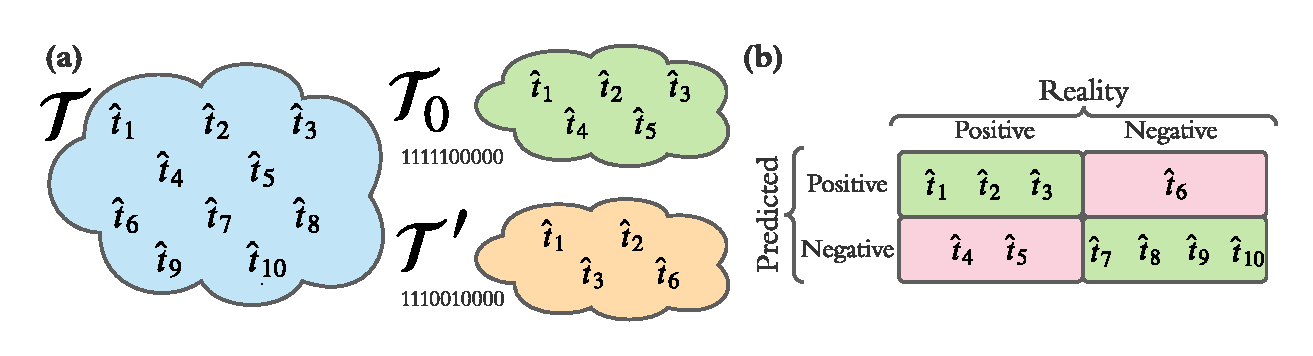
\includegraphics[width=\textwidth]{theoretical_study/figures/classication_example.pdf}
    \end{center}
    \caption[Classification concepts]{
        Concepts used for classification. 
        \textbf{a}, the set of available terms $\termset$ containing individual terms $\hat{t}_1$ to $\hat{t}_{10}$. 
        The \gls{true model} $\ho$ is constructed from the set $\termset_0$. 
        Suppose a candidate $\hp$ has the set $\termset^{\prime}$. 
        \textbf{b}, the confusion matrix for $\hp$. Correctly classified terms are \glsentrylong{tp} and \glsentrylong{tn} (green), 
            and incorrectly classified terms are \glsentrylong{fp} and \glsentrylong{tn} (red). 
    }
    \label{fig:classification_eg}
\end{figure}

\begin{algorithm}
    \caption{\gls{es} subroutine: \ttt{generate\_models} via genetic algorithm}
    \label{alg:ga_generate_models}
    \DontPrintSemicolon
    \KwIn{ $\nu$ \tcp*[1]{information about models considered to date}}\
    \KwIn{ $t$ \tcp*[1]{truncation rate}}\;
    \KwIn{ $g(\hi)$ \tcp*[1]{objective function that can act on any model $\hi$}}\;

    \KwOut{$\mathbb{H}$ \tcp*[1]{set of models}}\;
    
    $ N_m = \left| \nu \right| $ \tcp*[1]{number of models}

    \For{$\hi \in \nu$}{
       $g_i \gets g(\hi)$ \tcp*[1]{model fitness via objective function}
    }\;
    $r \gets $ \ttt{rank($\{ g_i \}$)} \tcp*[1]{rank models by their fitness}
    $\mathbb{H}_t \gets $ \ttt{truncate($r, N_m\times t$)} \tcp*[1]{truncate models by rank: only keep $N_m \times t$}
    $ s \gets $ \ttt{normalise($\{g_i\}$)} $\forall \hi \in \mathbb{H}_t$ \tcp*[1]{normalise remaining models' fitnesses}

    $\mathbb{H} = \{\}$ \tcp*[1]{new batch of chromosomes/models}

    \While{ $\left| \mathbb{H} \right| < N_m$ }{
        $p_1, p_2 = $ \ttt{roulette($s$)} \tcp*[1]{use $s$ to select two parents via roulette selection}
    
        $c_1, c_2$ = \ttt{crossover($p_1, p_2$)} \tcp*[1]{produce offspring models}

        $c_1, c_2$ = \ttt{mutate($c_1, c_2$)} \tcp*[1]{probabilistically mutate}

        $\mathbb{H} \gets \mathbb{H} \cup \{ c_1, c_2 \} $ \tcp*[1]{add new models to batch}

    }\;

    % \ttt{roulette($s$)}

    return $\mathbb{H}$ 

\end{algorithm}


\subsubsection{Distinguishing $\fs$ through Bayes factors}\label{sec:bf_by_f_score}
We have so far relied on \gls{bf} as the means by which to distinguish models' 
    ability to explain data from \gls{q}. 
We conjecture that models of higher $\fs$ are usually statistically better at predicting dynamics of \gls{q}
    than those of lower $\fs$, and therefore \glspl{bf} will favour models of higher $\fs$;
Verifying this hypothesis will allow us to incorporate statistical tools into the design of \glspl{of};
    we can perform straightforward tests training models of equally spaced $\fs$, and computing \glsentryshort{bf} between all pairs.
\par 

In \cref{fig:bf_by_fscore}, we show the relationships between $\fs$ and \gls{bf} for various conditions. 
Firstly, under a standard training regime with full \gls{bf} comparisons between all pairs, 
    we see that in most cases, the model with higher $\fs$ is favoured by \gls{bf}.
In \cref{fig:bf_by_fscore}b, we run a complete model training subroutine, but compute the \gls{bf} based on fewer experiments and particles 
    (retaining a fraction $\Np^{\prime} = 0.2\Np, \ \Ne^{\prime} = 0.2\Ne$ for comparisons).
This verifies an earlier claim from \cref{sec:experiments_for_bf}: 
    although the strength of evidence is weaker given reduced \gls{bf} resources, 
    the direction of the evidence is usually the same, i.e. the insight is indicative of the true physics, 
    so we can save considerable compute time by trusting these restricted \gls{bf} calculations. 
On the other extreme, we see in \cref{fig:bf_by_fscore}\textbf{c}, where models are trained with
    -- and \glspl{bf} based upon -- even greater resources than \cref{fig:bf_by_fscore}\textbf{a}, we see a similar effect: 
    adding resources strengthens the evidence, but does not fundamentally change the outlook. 
Finally, in addition to reducing the resources used per \gls{bf} calculation, 
    we reduce the number of comparisons computed in \cref{fig:bf_by_fscore}\textbf{d}, 
    as permitted when rating models according to the \gls{of} to be described in \cref{sec:elo}, 
    or similar measures which can yield fitnesses from reduced data. 
Essentially we can see that the insight is largely the same 
    from the most and least expensive training/comparison strategies, 
    and by leveraging the available evidence (\cref{fig:bf_by_fscore}\textbf{d}), 
    rather than brute-force computing as much evidence as possible (\cref{fig:bf_by_fscore}\textbf{a}), 
    we can achieve similar results. 
Note that the time saving reported between full and partial connectivity between models scales with $N_m$: 
    here, with $N_m=10$, the former computes 45 \glspl{bf}, while the latter computes 17;
    for $N_m=60$, as used in full instances/runs presented in this chapter, these rise to 600 and 1770 respectively, 
    so the benefit of the latter scheme is amplified. 
% This saving depends on the user's choice of graph connectivity, see \cref{sec:elo_graph}, 
%     though is typically a factor between 2-3;
%     in general, though, assuming we can reduce the resources used within the \gls{bf}, 
%     this phase is considerably less cumbersome than the model training itself, so 
%     it is feasible to compute all available \glspl{bf} to inform the \gls{bfeer}.

\begin{figure}
    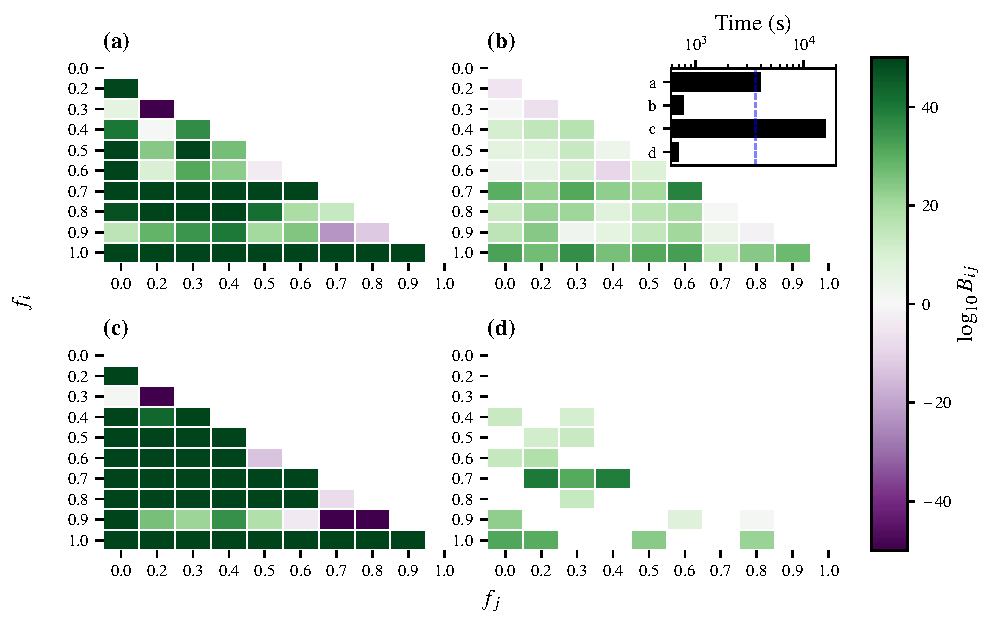
\includegraphics{theoretical_study/figures/bayes_factors_by_f_scores.pdf}
    \caption[\glsentrylong{bf} by $\fs$]{
        Pairwise \glsentrylong{bf}, $\bij$, by $\fs$ of candidates $\hi$ ($f_i$ on the $y$-axis) 
        and $\hj$ ($f_j$ on the $x$-axis).
        $\log_{10}\bij > 0 \ (<0)$, green (purple), indicates statistical evidence that $\hi$ ($\hj$) 
        is the better model with respect to the observed data.
        Visualisation is curtailed to $\log_{10} \bij = \pm 50$. 
        \textbf{a}, Models are trained with $\Ne=500, \Np=2500$,
            and all available data is used in the calculation of \glspl{bf}. 
        \textbf{b}, $\Ne=500, \Np=2500$ using only a fraction (0.2) of experiments/particles for \gls{bf} calculations. 
        \textbf{c}, $\Ne=1000, \Np=5000$, using all available data in the calculation of \glspl{bf}. 
        \textbf{d}, $\Ne=500, \Np=2500$, comparing only a subset of pairs of models through \glspl{bf}, 
            and using only a fraction ($0.2$) of experiments/particles for those calculations. 
            This pairwise comparison strategy is used for the \gls{of} in \cref{sec:elo}. 
        \textbf{Inset}, timings for each approach in seconds, with $t=1\textrm{hr}$ marked vertically in blue. 
        \figtableref
    }
    \label{fig:bf_by_fscore}
\end{figure}


\subsection{Hyperparameter search}
\label{sec:hyperparameter}
\begin{figure}
    \begin{center}
        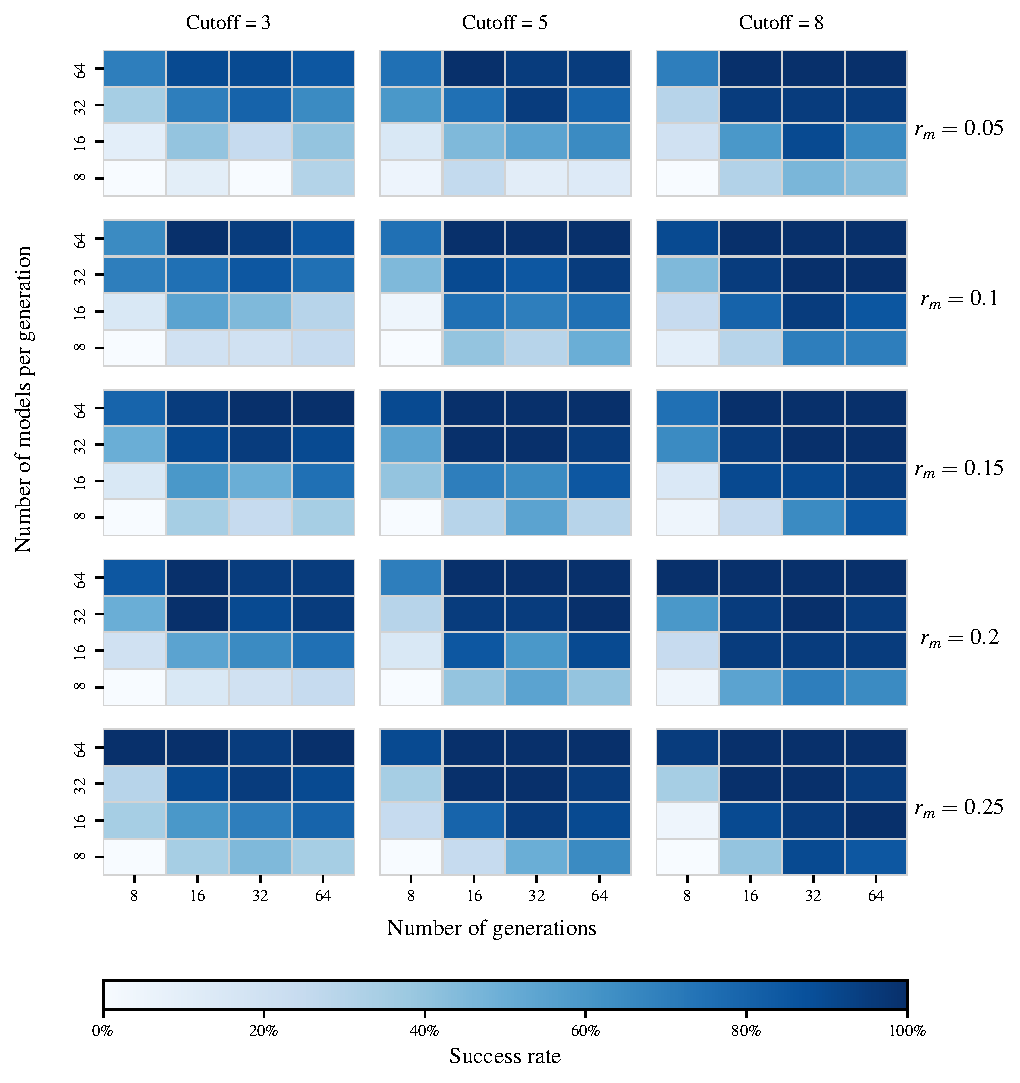
\includegraphics{theoretical_study/figures/gen_alg_param_sweep.pdf}
    \end{center}
    \caption[Genetic algorithm parameter sweep]{
        Genetic algorithm parameter sweep.
        Each subplot shows the success rates for varying numbers of generations, $N_G \in \{8, 16, 32, 64\}$, 
        and numbers of models per generation, $N_m \in \{8, 16, 32, 64\}$. 
        A subplot is generated for ranges of the mutation rate, $r_m$ and the number of 
        generations for which the elite model is unchanged after which the \gls{ga} is cut off.
        \figtableref 
    }
    \label{fig:ga_param_sweep}
\end{figure}

Firstly we will validate our reasoning that $\fs$ is a sensible figure of merit, 
    by directly invoking it as the \glsentrylong{of}. 
That is, we first implement a \gls{ga}, using the mapping between models and chromosomes outlined above,
    where we fix the numbers of sites $d=4$, and assume full connectivity between the sites, with $x-$, $y-$ and $z-$ couplings available,
        such that there are $N_t = 3 \times {4 \choose 2} = 18$ terms in $\termset$, so that the total population is of size $2^{18}$ chromosomes.
We can then sweep over the \gls{ga} \glspl{hyperparameter} to find a suitable configuration:
    in \cref{fig:ga_param_sweep} we show how the choice of parameters affect the success rate of preciesly identifying the 
    target chromosome, which is chosen at random for each instance, and we run 20 \glspl{instance} of each configuration. 
The studied hyperparameters\footnotemark \ are
\begin{easylist}[enumerate]
    \ListProperties(Numbers=r)
    & number of generations;
    & number of models per generation;
    & mutation rate, $r_m$;
    & number of generations for which a candidate must reign as the strongest observed, before the search terminates, the \emph{cutoff}. 
\end{easylist}
\footnotetext{  
    These and further \glspl{hyperparameter} can be swept using code within the \gls{qmla} codebase, 
    in the directory \ttt{scripts/genetic\_alg\_param\_sweep}.  
}
Naturally, we expect that running for more generations with more models per generation will result in a more effective search in the model space, 
    having examined $N_gN_m$ models. 
We must also consider, however, that -- in realistic cases of \gls{qmla} -- the total computation time scales dramatically with these parameters, 
    since training and comparing models are expensive subroutines. 
Our goal is therefore to identify the set of \glspl{hyperparameter} which best searches the \gls{model space} 
    while demanding the lowest $N_g, N_m$.  
We see that, unsurprisingly, the \gls{ga} performs poorly when run with few resources, 
    but broadly the performances are similiar provided it is run with sufficient resources.
We can bound the parameters $r_m \geq 0.1, \textrm{cutoff} \geq 5, N_m \geq 16, N_g \geq 16$ to ensure a reasonable 
    search through the model space, without having to consider a prohibitive number of models. 
We must bear in mind, however, that this parameter sweep refers only to the trivial case where 
    the $\fs$ is used as the \gls{of}, so we do not expect such high success rates in realistic cases.

\section{Objective functions}\label{sec:objective_functions}
\glsreset{of}
We have alluded to the central probelm in building a \gls{ga} into \gls{qmla}:
    how to evaluate trained candidate models in the absence of a natural \gls{of}. 
In \crefrange{sec:inverse_ll}{sec:elo} we will propose and analyse a number of potential \glspl{of}, 
    some of which will underlie later studies in this thesis. 
We conclude this study by comparing the proposed \glspl{of} and selecting one for consideration in the remainder of this chapter;
    readers interested in the final application may prefer to skip to \cref{sec:obj_fnc_selection}.
\par 
We will show how each \gls{of} computes a fitness, $g_i$, for candidate models, $\hi$.
For examples of each, we group together some demonstrative values in \cref{table:objective_functions}.
For each $\hi$, we may refer to 
\begin{easylist}[itemize]\label{list:obj_fnc_terms}
    & $\tll_i$, \glsentryfull{tltl},  introduced in \cref{sec:total_log_total_likelihood};
    & $k_i$, the model's cardinality, i.e. number of terms in its parameterisation;
    & $\expset_i$, the bespoke set of experiments composed by the \glsentrylong{edh} (\cref{sec:heuristic}) solely for trainng $\hi$;
    & $n = |\expset_i|$, the number of samples (datapoints) used in trainng $\hi$. 
\end{easylist}
In \cref{table:objective_functions}, 
    we consider six randomly generated exemplary models 
    -- of varying quality with respect to the target, $\ho$, listed in \cref{eqn:obj_fnc_eg_models} -- 
    to demonstrate each \gls{of}'s outcomes.

\renewcommand{\arraystretch}{1.25} % space between rows
\setlength{\tabcolsep}{2pt}

\begin{equation}
    \label{eqn:obj_fnc_eg_models}
    \begin{align}
        \hat{H}_0 \ &= \ \s_{(1, 2)}^{z}\s_{(1, 3)}^{z}\s_{(2, 3)}^{z}\s_{(2, 5)}^{z}\s_{(3, 5)}^{z};\\
        \hat{H}_a \ &= \ \s_{(1, 5)}^{z}\s_{(3, 4)}^{z}\s_{(4, 5)}^{z}; \\
        \hat{H}_b \ &= \ \s_{(1, 4)}^{z}\s_{(1, 5)}^{z}\s_{(2, 5)}^{z}\s_{(3, 4)}^{z}; \\
        \hat{H}_c \ &= \ \s_{(1, 2)}^{z}\s_{(1, 5)}^{z}\s_{(2, 4)}^{z}\s_{(2, 5)}^{z}\s_{(4, 5)}^{z}; \\
        \hat{H}_d \ &= \ \s_{(1, 3)}^{z}\s_{(1, 4)}^{z}\s_{(1, 5)}^{z}\s_{(2, 4)}^{z}\s_{(2, 5)}^{z}\s_{(3, 4)}^{z}\s_{(3, 5)}^{z}; \\
        \hat{H}_e \ &= \ \s_{(1, 2)}^{z}\s_{(1, 3)}^{z}\s_{(1, 5)}^{z}\s_{(2, 3)}^{z}\s_{(2, 5)}^{z}\s_{(4, 5)}^{z}; \\
        \hat{H}_f \ &= \ \s_{(1, 2)}^{z}\s_{(1, 3)}^{z}\s_{(2, 3)}^{z}\s_{(2, 4)}^{z}\s_{(2, 5)}^{z}\s_{(3, 4)}^{z}\s_{(3, 5)}^{z}. \\
    \end{align}
\end{equation}

\begin{table}    
    \begin{tabular}{|cc|c|c|c|c|c|c|}
\hline
          &      &                              $\hat{H}_a$ &                              $\hat{H}_b$ &                              $\hat{H}_c$ &                              $\hat{H}_d$ &                              $\hat{H}_e$ &                              $\hat{H}_f$ \\
Method &  &                                          &                                          &                                          &                                          &                                          &                                          \\

          & $F_1$ &                                    $0.0$ &                                    $0.2$ &                                    $0.4$ &                                    $0.5$ &                                    $0.7$ &                                    $0.8$ \\
          & $k$ &                                        3 &                                        4 &                                        5 &                                        7 &                                        6 &                                        7 \\
          & $\overline{l_e}$ &                          $0.86 \pm 0.29$ &                          $0.84 \pm 0.29$ &                          $0.77 \pm 0.27$ &                          $0.78 \pm 0.29$ &                          $0.79 \pm 0.26$ &                          $0.79 \pm 0.26$ \\
          & $\tll_i$ &                                     -143 &                                     -152 &                                     -131 &                                     -150 &                                     -125 &                                     -124 \\
\hline \multirow{2}{*}{Inverse log-likelihood} & $g_i^L$ &                                  0.00698 &                                  0.00659 &                                  0.00766 &                                  0.00669 &                                  0.00803 &                                  0.00804 \\
          & $\%$ &                                       23 &                                        0 &                                       25 &                                        0 &                                       26 &                                       26 \\
\cline{1-8}
\hline \multirow{5}{*}{Akaike Info Criterion} & AIC &                                      293 &                                      311 &                                      271 &                                      313 &                                      261 &                                      263 \\
          & AICc &                                      293 &                                      312 &                                      272 &                                      314 &                                      262 &                                      264 \\
          & $w_i^A$ &                                 1.81e-07 &                                  1.4e-11 &                                  0.00724 &                                 4.15e-12 &                                        1 &                                    0.334 \\
          & $g_i^A$ &                                 1.17e-05 &                                 1.03e-05 &                                 1.35e-05 &                                 1.01e-05 &                                 1.46e-05 &                                 1.43e-05 \\
          & $\%$ &                                       22 &                                        0 &                                       25 &                                        0 &                                       27 &                                       26 \\
\cline{1-8}
\hline \multirow{4}{*}{Bayesian Info Criterion} & BIC &                                      301 &                                      322 &                                      284 &                                      331 &                                      277 &                                      281 \\
          & w_i^B &                                 5.49e-66 &                                 1.26e-70 &                                 1.97e-62 &                                 1.11e-72 &                                 8.43e-61 &                                 8.95e-62 \\
          & g_i^B &                                 1.11e-05 &                                 9.65e-06 &                                 1.24e-05 &                                 9.11e-06 &                                 1.31e-05 &                                 1.27e-05 \\
          & $\%$ &                                       23 &                                        0 &                                       25 &                                        0 &                                       27 &                                       26 \\
\cline{1-8}
\hline \multirow{2}{*}{Bayes factor points} & g_i^p &                                        0 &                                        2 &                                        3 &                                        2 &                                        3 &                                        5 \\
          & $\%$ &                                        0 &                                       13 &                                       20 &                                       13 &                                       20 &                                       33 \\
\cline{1-8}
\hline \multirow{3}{*}{Ranking points} & Ranking &                                        6 &                                        5 &                                        2 &                                        4 &                                        3 &                                        1 \\
          & g_i^R &                                        0 &                                        0 &                                      0.3 &                                      0.1 &                                      0.2 &                                      0.4 \\
          & $\%$ &                                        0 &                                        0 &                                       30 &                                       10 &                                       20 &                                       40 \\
\cline{1-8}
\hline \multirow{3}{*}{Elo rating} & Rating &                                      909 &                                      944 &                                     1042 &                                     1007 &                                     1011 &                                     1084 \\
          & g_i^E &                                        0 &                                       35 &                                      133 &                                       98 &                                      102 &                                      175 \\
          & $\%$ &                                        0 &                                        0 &                                       26 &                                       19 &                                       20 &                                       34 \\
\cline{1-8}
\hline \multirow{3}{*}{Residuals} & mean$\{\tilde{r_p^e}\}$ &                                    0.132 &                                    0.146 &                                    0.114 &                                    0.138 &                                   0.0858 &                                   0.0715 \\
          & g_i^r &                                    0.753 &                                    0.729 &                                    0.785 &                                    0.743 &                                    0.836 &                                    0.862 \\
          & $\%$ &                                       23 &                                        0 &                                       24 &                                        0 &                                       26 &                                       27 \\
\hline
\end{tabular}
 % TODO fix latex errors in table
    \caption[Objective function examples]{
        Examples of how each objective function, $g$ as described in \cref{sec:inverse_ll} to \cref{sec:elo},
            assign selection probability (denoted \%) to the same set of candidate models, $\{\hi\}$ listed in \cref{eqn:obj_fnc_eg_models}, 
            when attempting to learn data from $\ho$. 
        Intermediate quantities, e.g. $w_i^A$, $g_i^p$ are described in the section of the main text describing the corresponding \gls{of}.
        For each model we first summarise its
            $\fs$ (\cref{eqn:f1_score}),
            number of terms $k$,
            median  \gls{likelihood} $\overline{l_e}$ (\cref{eqn:log_likelihood}),     
            and \gls{tltl} $\tll_{i}$ (\cref{eqn:log_total_likelihood}), 
        We use $n=250$ samples, i.e. $\tll_{i}$ is a sum of $n$ \glspl{likelihood} .  
        The set of models is truncated so that only the strongest four are assigned selection probability. 
    }
    \label{table:objective_functions}
\end{table}

\subsection{Inverse log-likelihood}\label{sec:inverse_ll}
$\tll_{i}$, defined in \cref{eqn:log_total_likelihood}, can be thought of as a measure of the success of a given model at explaining data from any set of experiments, $\expset$. 
This can be immediately interpreted as an \gls{of}, provided each candidate model 
    computes a meaningful \gls{tltl}, requiring that they are all based on the same set of experiments, $\expset_v$,
    which are designed explicitly for the purpose of model evaluation. 
\par 

\gls{tltl} are negative and the strongest model has lowest $\lvert \tll_{i} \rvert$ (or highest $\tll_{i}$ overall),
    so the corresponding \gls{of} for candidate $\hi$ is 
\begin{equation}
    \label{eqn:obj_log_likelihood}
    g_i^{L} = \frac{-1}{\tll_{i}}.
\end{equation}

In our tests, Eqn. \ref{eqn:obj_log_likelihood} is found to be too generous to poor models, 
    assigning them non-negligible probability. 
Its primary flaw, however, is its reliance on $\expset_v$: 
    in order that the \gls{tltl} is significant, it must be based on meaningful experiments, 
    the design of which can not be gauranteed in advance, or at least risks introducing strong bias
    towards some models. 

\subsection{Akaike information criterion}\label{sec:akaike_info_criterion}
A common metric in the general field of model selection is \gls{aic} \cite{dr2002model}.
Incorporating \gls{tltl}, 
    \gls{aic} objectively quantifies how well a given model accounts for data from the target system,
    and explicitly punishes models which use extraneous parameters by incurring a penalty on $k_i$. 
\gls{aic} is given by 
\begin{equation}
    \label{eqn:aic}
    AIC_i = 2k_i - 2 \tll_{i}.
\end{equation}

In practice we use a slightly modified form of Eqn. \ref{eqn:aic} which
    corrects for the number of samples $n=\lvert\expset_i\rvert$, 
    called the \gls{aicc}, 
\begin{equation}
    \label{eqn:aicc}
    AICC_i = AIC_i + 2k_i \frac{k_i+1}{n-k_i-1}. 
\end{equation}

Model selection from a set of candidates occurs simply by selecting the model with lowest $AICC$.
Following \cite{dr2002model}, by using Eqn. \ref{eqn:aicc} as a measure of \emph{relative likelihood}
    we retrieve selection probability via
    the \emph{Akaike weights},
\begin{equation}
    \label{eqn:akaike_weights}
    w_i^A = \exp \left( \frac{{AICC_{\textrm{min}} - AICC_i}}{2} \right), 
\end{equation}
    where $AICC_{\textrm{min}} = \min_{i}\{ AICC_i\}$.

Akaike weights impose quite strong penalties 
    on models which do not explain the data well, 
    but also punish models with extra parameters, i.e. overfitting models, 
    effectively searching for the strongest and simplest model simultaneously.
The level of punishment for poorly performing models is likely too drastic: 
    very few models will be in a range sufficiently close to $AICC_{\textrm{min}}$ 
    to receive a meaningful Akaike weight, 
    suppressing diversity in the model population.
    Indeed, we can see from Table \ref{table:objective_functions} that this results in most 
    models being assigned negligible weight, which is not useful for parent selection. 
Instead we compute a straightforward quantity related to \gls{aic},
\begin{equation}
    \label{eqn:akaike_fitness}
    g_i^{A} = \left(\frac{1}{AICc_i}\right)^2,
\end{equation}
    where we square the inverse \gls{aicc} to amplify the difference in quality between models, 
    such that stronger models are rewarded.

\par 

\subsection{Bayesian information criterion}\label{sec:bayes_info_criterion}
Related to the concept of \gls{aic} (Eqn. \ref{eqn:aic}), is that of \gls{bic}, 
\begin{equation}
    \label{eqn:bic}
    BIC_i = k_i \ ln(n_i) - 2 \tll_{i},
\end{equation}
    where $k_i, n_i$ and $\tll_i$ are as defined on \cpageref{list:obj_fnc_terms}.
    % where $k, \tll_{i}$ are as defined above and $n$ is the number of samples.
Analagously to Akaike weights, 
    \emph{Bayes weights} as proposed in \S7.7 of \cite{friedman2001elements}, are given by

\begin{equation}
    w_i^B = \exp\left( - \frac{BIC_i}{2}  \right).
\end{equation}

\gls{bic} is harsher than \gls{aic} in its punishment of models' cardinality $k_i$, 
    demanding substantial statistical justification for the inclusion of more parameters. 
Again, this may be overly cumbersome for our use case:
    with such a relatively small number of parameters, 
    the punishment is disproportionate.
As with Akaike weights, rather than using Bayes weights directly, 
    we opt for an \gls{of} related to them, 
\begin{equation}
    \label{eqn:bic_fitness}
    g_i^B = \left( \frac{1}{BIC_i}\right)^2.
\end{equation}
    

\subsection{Bayes factor points}\label{sec:bf_points}
A cornerstone of model selection within \gls{qmla} is the calculation of \glspl{bf} (see \cref{sec:bayes_factors}). 
We can compute the pairwise \gls{bf} between two candidate models, $\bij$, according to Eqn. \ref{eqn:bf_succinct}.
$\bij$ can be based on some evaluation dataset, $\expset_v$, but can also be calculated from $\expset_i \cup \expset_j$: 
    this is a strong advantage since the resulting insight (Eqn. \ref{eqn:bf_cases}) is based on 
    experiments which were bespoke to both $\hi, \hj$. 
As such we can be confident that this insight accurately points us to the stronger of two candidate models. 
\par 

We can utilise this facility by computing the \gls{bf} between all 
    pairs of models in a set of $N_m$ candidates $\{\hi\}$, 
    i.e. compute ${N_m \choose 2}$ \gls{bf}s. 
Note that this is computationally expensive: 
    in order to train $\hi$ on $\expset_j$ requires a further $\lvert \expset_j \rvert$ experiments, 
    each requiring $N_P$ particles\footnote{Caveat the reduction in overhead outlined in \cref{sec:experiments_for_bf}.}, 
    where each particle corresponds to a unitary evolution and therefore the caluclation of a matrix exponential. 
The size of the \gls{model space} is then quite a heavy disadvantage: 
    examining $N_g$ generations requires $N_g \times {N_m \choose 2}$ \gls{bf} calculations for complete assessment. 
In the case where all pairwise \gls{bf} are performed, 
    we can assign a point to $\hi$ for every comparison in which it is deemed superior, according to \cref{eqn:bf_cases}.
\begin{equation}
    \label{eqn:bf_points}
    g_i^p = \sum_{j \in \mu} b_{ij}, \ \ \ \ b_{ij} = 
        \begin{cases}
            1, \ \ \ \ \bij > 1 \\
            0, \ \ \ \ \text{otherwise}.
        \end{cases}
\end{equation}
This is a straightforward mechanism, but is overly blunt
    because it does not account for the strength of the evidence
    in favour of each model. 
For example, a dominant model will receive only a slightly higher selection probability 
    than the second strongest, even if the difference between them was $\bij = 10^{100}$. 
Further, the unfavourable scaling make this an expensive method. 

\subsection{Ranking}\label{sec:bf_ranking}
Related to \cref{sec:bf_points}, we can rank models in a generation based on their number of \gls{bf} points.
\gls{bf} points are assigned as in Eqn. \ref{eqn:bf_points}, 
    but instead of corresponding directly to fitness, 
    we assign models a rank $R$, 
    i.e. the model with highest $g_i^p$ gets $R=1$, 
    and the model with $n^{th}$ highest $g_i^p$ gets $R=n$. 
Note here we truncate $\mu$, meaning we remove the worse-performing models and retain only $N_m^{\prime}$ models, 
    before calculating $R$, because computing $R$ using all $N_m$ models results in less distinct selection probabilities. 

\begin{equation}
    \label{eqn:ranking}
    g_i^R = \frac{N_m^{\prime}-R_i+1}{\sum\limits_{n=1}^{N^{\prime}_m} n},
\end{equation}
    where $R_i$ is the ranking of $\hi$ and $N_m^{\prime}$ is the number of models retained after truncation. 
\cref{eqn:ranking} has a similary effect to \cref{eqn:bf_points} but awards higher selection probability to 
    the strongest models. 
However, it too overlooks the nuanced perspective available through the total statistical evidence gathered by the series of \glspl{bf}. 

\subsection{Residuals}\label{sec:residuals}
Recall at each experiment, $N_P$ particles are compared against a single experimental datum, $d$. 
By definition, $d$ is the binary outcome of the measurement on \gls{q} under experimental conditions $e$.
That is, $d$ encodes the answer to the question: 
    after time $t$ under Hamiltonian evolution, did \gls{q} project onto 
    the basis we have labelled $\ket{d}$ (usually the same as the input \gls{probe} state $\ket{\psi}$)?
\par 
In practice we often have access to the complete \gls{likelihood}, 
    i.e. rather than a binary value, we have a number representing the probability that 
    \gls{q} will project on to $d=0$ for a given experiment $e$, $\Pr_Q(0 | e)$. 
The likelihood -- in this case equivalent to the expectation value -- 
    for \gls{q} is usually given by $\absval{ \bra{\psi} e^{-i\ho t} \ket{\psi} }^2$.
For consistency with QInfer \cite{qinfer-1_0} -- on which \gls{qmla}'s code base extends --
    we call the expectation value for the system $\Pr_Q(0)$;
    the same quantity can be computed for each particle, called $\Pr_p(0)$.
Likewise, we can simulate this quantity for each particle, $\Pr_p(0 | e)$. 
This allows us to calculate the \emph{residual} between the system and individual particles' \glspl{likelihood}, $r_p^e$; 
    we can hence compute the mean residual across all particles in a single experiment $r^e$:
\begin{align}
    \label{eqn:particle_residual}
    \begin{split}
    r_p^e & = \absval{ Pr_Q(0 | e) - Pr_p(0 | e) }  \\
    r^e &= \underset{p}{\text{mean}} \{r_p^e\}
    \end{split}
\end{align}
\par 

Residuals capture how closely the particle distribution reproduced the dynamics from \gls{q}:
    $r^{e}_{p} = 0$ indicates perfect preditiction, while $r^e_p=1$ is completely incorrect. 
We can therefore maximise the quantity $1-r$ to find the best model, 
    using the \gls{of}
\begin{equation}
    \label{eqn:residual_fitness}
    g^r_i = \lvert 1 - \underset{e \in \expset}{\text{mean}}\{ {r^e} \}\rvert^2.
\end{equation}
\par     
This \gls{of} can be thought of in frequentist terms 
    as similar to the residual sum of squares,
    although instead of summing the residual squares, we take the average to ensure $0 \leq r \leq 1$. 
$g_i^r$ encapsulates how well the candidate model reproduces a paticular set of dynamics from the target system, 
    as a proxy for how well that candidate describes the system. 
This is not always a safe figure of merit: 
    in most cases, we do not expect parameter learning to perfectly optimise $\al_i$. 
Reproduced dynamics alone can not capture the prospect that $\hi=\ho$, 
    but rather inform statistical measures such as \gls{bf} that allow us to make 
    qualified statements about the system. \par 

This \gls{of} provides a useful test for \gls{qmla}'s \gls{ga}:
    by simulating the case where parameters \emph{are} learned perfectly, 
    such that we know that $g_i^r$ truly represents the ability of $\hi$ to 
    simulate $\ho$, then this \gls{of} gaurantees to promote  the strongest models,
    especially given that $\hi=\ho \implies r_p^e=0 \ \forall \ \{e, p\}$. 
In realistic cases, however, the non-zero residuals -- even for 
    strong $\hi$ -- may arise from imperfectly learned parameters,
    rendering the usefulness of this \gls{of} uncertain. 
Finally, it does not account for the cardinality, $k_i$, of the candidate models,
    which all \gls{ml} protocols aim to avoid in general;
    this could result in favouring severely overfitting models in order to 
    gain marginal improvement in residuals.

\subsection{Bayes factor enhanced Elo-ratings}\label{sec:elo}
A popular tool for rating individual competitors in sports and games is the \emph{Elo rating} scheme, 
    e.g. used to rate chess players and soccer teams \cite{elo1978rating, fifa_elo}, 
    also finding application in the study of animal hierarchies \cite{neumann2011assessing}. 
Elo ratings allow for evaluating the relative quality of individuals 
    based on incomplete pairwise competitions, 
    e.g. despite two football teams having never played against each other before, 
    it is possible to quantify the difference in quality between those teams, 
    and therefore to predict a result in advance \cite{hvattum2010using}. 
There is a direct a parallel between these types of competitions and \gls{qmla}:
    we similarly have a pool of individual competitors (models), 
    which we can place in direct competition, 
    and quantify the comparitive outcome through \gls{bf}, 
    in order to determine the strongest. 

\par 
Elo ratings are transitive: given some interconnectivity in a generation, 
    we need not compare \emph{every} pair of models in order to 
    make meaningful claims about which are strongest;
    it is sufficient to perform a subset of comparisons, 
    ensuring each individual undergoes robust competition.
We can take advantage of this transitivity to reduce the combinatorial overhead 
    usually associated with computing bespoke \glspl{bf} between all models 
    (i.e. using their own training data $\expset_i$ instead of a generic 
    $\expset_v$).
In practice, we map $N_m$ models within a generation to vertices on a regular graph
    of degree $nicefrac{N_m}{3}$, i.e. each model is connected to $\nicefrac{N_m}{3}$ 
    other models within $\mu$. 
Models which share an edge then undergo \gls{bf} comparison. 
For example, with $N_m=60$ this leads to $600$ \gls{bf} calculations, 
    compared with $1770$ calculations in the fully connected graph. 
While every pair of models $(\hi, \hat{H}_{m})$ are not directly connected, 
    there is always a chain of length $l \leq l_{max}$ edges between them.
For $N_m=60$, we find $l_{max}=2$, 
    e.g. for $\hi, \hat{H}_k$ disconnected, there are comparisons $(\hi, \hj), (\hj \hat{H}_k)$. 
    
\par 

The Elo rating scheme is a nonlinear points transfer system, as follows: 
    upon creation, $\hi$ is assigned a rating $R_i$; 
    every comparison with a competitor $\hj$ results in $\bij$; 
    $R_i$ is updated according to the known strength of its competitor, $R_j$, 
    as well as the result $\bij$. 
The Elo update ensures that winning models are rewarded 
    for defeating another model, 
    but that the extent of that reward reflects the quality of its opponent. 
As such, this is a fairer mechanism than \gls{bf} points, 
    which award a point for every victory irrespective of the opposition:
    if $\hj$ is already known to be a strong or poor model, 
    then $\Delta R_i$ proportionally changes the credence we assign to $\hi$. 
It achieves this by first computing the \emph{expected} result of a given comparison
    with respect to each model, based on the current ratings, 

\begin{subequations}
    \label{eqn:elo_expected_score}
    \begin{equation}
        E_i 
        = \frac{1}{1 + 10^{\frac{R_j - R_i}{400}}} ;
    \end{equation}
    \begin{equation}
        E_i + E_j = 1,
    \end{equation}    
\end{subequations}

Then, we find the binary \emph{score} from the perspective of each model,
\begin{equation}
    \label{eqn:elo_score}
    \begin{cases}
        B_{ij} > 1 & \Rightarrow \ S_i = 1; \ S_j =0  \\
        B_{ij} < 1 & \Rightarrow \ S_i = 0; \ S_j = 1 \\
    \end{cases}
\end{equation}
which is used to determine the change to each model's rating,
\begin{equation}
    \label{eqn:elo_delta_r}
    \Delta R_i = \eta \times \left( S_i - E_i \right).
\end{equation}

An important detail is the choice of $\eta$, i.e. the \emph{weight} of the 
    change to the models' ratings. 
In standard Elo schemes this is a fixed constant, 
    but here -- taking inspiration from football ratings where $\eta$ is the number of goals 
    by which one team won -- we weight the change by the strength of our belief in the outcome: 
    $\eta \propto \lvert \bij \rvert$.
That is, similarly to the interpretation of Eqn. \ref{eqn:bf_cases}, 
    we use the evidence in favour of the winning model to transfer points from the loser to the winner,
    albeit we temper the effect by instead using $\eta = \log_{10}(B_{ij})$, since \gls{bf} can give very large numbers. 
In total, then, following the comparison between models $\hi, \hj$, we can perform the Elo rating update
\begin{equation}
    \label{eqn:elo_update}
    R_i^{\prime} = R_i + \log_{10}(B_{ij}) \left(S_i - \frac{1}{1 + 10^{\frac{R_j - R_i}{400}}}\right).
\end{equation}
This procedure is easiest to understand by following the example in Table \ref{table:elo_eg}. 

\begin{table}
    \centering
    \begin{tabular}{|cc|c|c|c|c|c|c|c|}
    \hline
                            &             &                                    $R_i$ &                                    $E_i$ &                                    $S_i$ &                                 $B_{ij}$ &                       $\log_{10}(B_{ij})$ &                             $\Delta R_i$ &                           $R_i^{\prime}$ \\
     & Model &                                          &                                          &                                          &                                          &                                          &                                          &                                          \\
    % \hline
    \hline \multirow{2}{*}{$\hat{H}_a > \hat{H}_b$} & $\hat{H}_a$ &                                     1000 &                                     0.76 &                                        1 &                                   1e+100 &                                      100 &                                     0.24 &                                   1024.0 \\
                            & $\hat{H}_b$ &                                      800 &                                     0.24 &                                        0 &                                   1e-100 &                                      100 &                                    -0.24 &                                    776.0 \\
    \cline{1-9}
    \hline \multirow{2}{*}{$\hat{H}_b > \hat{H}_a$} & $\hat{H}_a$ &                                     1000 &                                     0.76 &                                        0 &                                   1e-100 &                                      100 &                                    -0.76 &                                    924.0 \\
                            & $\hat{H}_b$ &                                      800 &                                     0.24 &                                        1 &                                   1e+100 &                                      100 &                                     0.76 &                                    876.0 \\
    \hline
    \end{tabular}
    
    \caption[Example of Elo rating updates]{
        Example of Elo rating updates. 
        We have two models, where $\h_a$ is initially believed to be a stronger candidate than $\h_b$, 
            i.e. has a higher starting Elo rating, $R_i$.     
        We demonstrate the effect when there is strong evidence\footnotemark \ in favour of either model through \gls{bf} comparison, $\bij \sim 10^{100}$. 
        In the first case, $\h_a$ defeats $\h_b$, as firmly expected according to their initial ratings,
            so the corresponding reward (cost) for $\h_a$ ($\h_b$) is relatively small.
        In the second case, contrary to prediction $\h_b$ outperforms $\h_a$, 
            so $\h_b$ receives a large share of Elo points from $\h_a$. 
    }
    \label{table:elo_eg}
\end{table}
\footnotetext{
    Note to achieve $\bij = 10^{100} = e^{\tll_{i} - \tll_{j}} \implies \tll_{i} - \tll_{j} = ln(10^{100}) \approx 7$.
}


\par 
Finally, it remains to select the starting rating $R_i^0$ to assign models upon creation. 
Although this choice is arbitrary, it can have a strong effect on the progression of the algorithm. 
Here we impose details specific to the \gls{qmla} \gls{ga}: 
    at each generation we admit the top two  models automatically 
    for consideration in the next generation, 
    such that strongest models can stay alive in the population and ultimately win. 
These are called \emph{elite} models, $\hat{H}_e^1, \hat{H}_e^2$. 
This poses the strong possibility for a form of generational wealth:
    if elite models have already existed for several generations, 
    their Elo ratings will be higher than all alternatives by defintion. 
Instead, we would prefer that newly spawned models can overtake the Elo rating of elite models. 
To resolve this, at each generation, all models -- including $\hat{H}_e^1, \hat{H}_e^2$ -- 
    are assigned the same initial rating, $R_i^0=1000$. 

% We achieve this through an imprecise mechanism:
%     newly born models are given the Elo rating of the second-most-elite model, $\h_e^2$. 
% This performs three key functions: 
% \begin{easylist}[enumerate]
%     \ListProperties(Numbers=r)
%     & new models are immediately \emph{within range} of the elite models; 
%     if they perform well enough, they have a realistic and fair chance of overtaking them; 
%     & the strongest model retains some of its advantage gained over previous generations 
%     -- in order that the ratings are meaningful, there must be some advantage accrued over series of victories; 
%     & $\hat{H}_e^2$ is allowed continue to compete, but has no advantage:
%     in order to retain its status as elite, it must perform well \emph{again} in this generation,
%     so it can not simply rely on results from previous generations -- against inferior opposition -- 
%     to remain active in the gene pool. 
    
% \end{easylist}

\par 
In order to derive a meaningful selection probability for each candidate, 
    we must first ground the raw Elo rating at each generation $\mu$:
    we subtract the lowest rating among the entertained models, $R_{\textrm{min}}^{\mu}$.
This serves to ensure the range of remaining $R_i$ represent only by the difference between
    models as assessed within $\mu$: 
    a very strong model might have much higher $R_i$ than its contemporaries, 
    but that difference was earned exclusively by comparison within $\mu$, 
    so it is deserving of its higher fitness and therefore greater selection probability. 
We perform this step before truncation\footnotemark, so that the models remaining post-truncation
    all have non-zero fitness. 
Finally, then, we name this \gls{of} the \emph{\gls{bfeer}}:
    the fitness of each model $\hi^{\mu} \in \mu$ is attained directly from its rating $R_i$
    after undergoing Elo updates based on \glspl{bf} in the current generation, minus the minimum rating of any model 
    in the same generation $R^{\mu}_{\textrm{min}}$,
\footnotetext{
    We truncate the $N_m$ models on $\mu$ by the truncation rate $\tau$,
    i.e. only $\tau N_m$ models are considered as potential parents in the \gls{ga}.
    In this chapter we use $\tau=\nicefrac{1}{3}$.
}

\begin{equation}
    \label{eqn:elo_fitness}
    g_i^E = R_i^{\mu} - R_{\textrm{min}}^{\mu}.
\end{equation}
The advantage of this \gls{of} is that it gives a meaningful value on the absolute quality of every model, 
    allowing us to determine the strongest, and importantly to find the relative strength between models. 
Further, it exploits bespoke \glspl{bf}, i.e. based on the considered models' 
    individually designed $\expset_i$,
    removing the impetus to design $\expset_v$ which can
    evaluate models definitively. 
One disadvantage is that it does not explicitly punish models based 
    on their cardinality, 
    however this feature is partially embedded by adopting \gls{bf} for the comparisons, 
    which are known to protect against overfitting \cite{kass1995bayes}.

\subsection{Objective function selection}\label{sec:obj_fnc_selection}
\begin{figure}
    \centering
    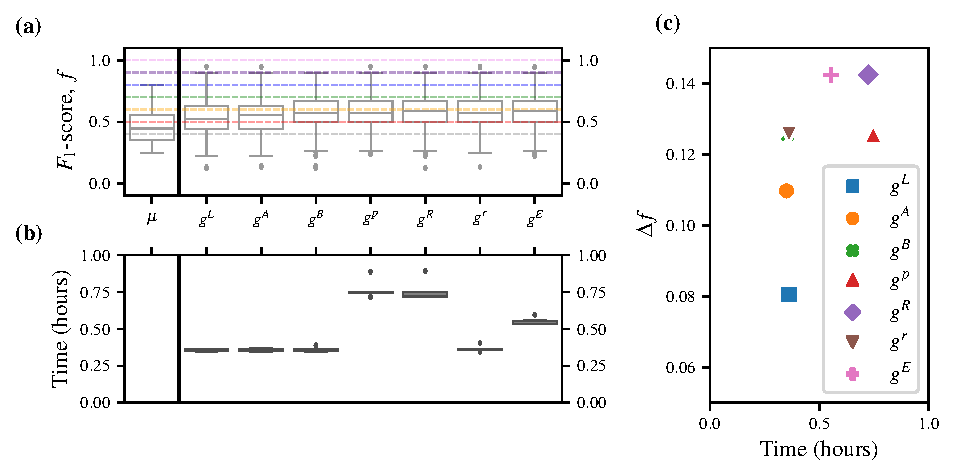
\includegraphics[width=0.95\textwidth]{theoretical_study/figures/objective_fnc_comparison.pdf}
    \caption[Comparison between proposed \glsentrylongpl{of}]{
        Comparison between proposed \glsentryfullpl{of}. 
        Each \gls{of} trains the same initial generation of $N_m=28$ models with resources
        $N_E=500, N_P=2000$, and then design a new set of $N_m$ models through 
        a roulette strategy, such that the only difference between \gls{of}'s output 
        is how they assign selection probability.
        We run each \gls{of} 25 times for the same target system, 
            a $4$--qubit Heisenberg--XYZ model. 
        \textbf{(a)} shows the box--plot of spawned models' \fs, \ $f$, 
            where the median and inter--quartile ranges are indicated by the boxes,
            as well as those of the initial generation $\mu$ centered on $f_{\mu}=0.45$.
            We mark $f=\{0.4, 0.5, ..., 1.0\}$ for ease of interpretation. 
        \textbf{(b)} shows box--plots of the time taken to compute the single generation in each case.
        In \textbf{(c)} we report the difference between the median $f$ among the 
            newly proposed models from $f_{\mu}$, $\Delta f$,
            plotted against the time to achieve the result. 
    }
    \label{fig:obj_fnc_comparison}
\end{figure}

Having proposed a series of possible objective functions, 
    we are now in a position to analyse their appropriateness in the context of \gls{qmla}. 
Recall from \cref{sec:f_score} that we use \fs as the figure of merit against which individual models are measured;
    we can compare \glspl{of} on the basis of the \fs of models they spawn.

\par 

First we can remark on the examples listed in \cref{table:objective_functions}. 
The \glspl{of} which rely on the \gls{tltl}, i.e. $g^L, g^A, g^B, g^r$, 
    are effectively tricked by the log-likelihood, which appears reasonably convincing for 
    poor models, e.g. $\h_a, \h_c$. 
This underlines the risk in buidling $\expset_v$, which can be biased towards weak models, 
    for example resulting in high selection probability for $\h_a$ which has $f=0$, 
    while $\h_d$, with $f=0.4$ is discarded. 
On the other hand, \glspl{of} grounded by the \gls{bf} ($g^p, g^R, g^E$) invariably 
    promote models of higher $\fs$, justifying the role of statistical evidence 
    used for those calculations. 
Overall, however, the insights from this complete example are insufficient to 
    make general claims about the performance of each \gls{of}, 
    so here we examine their outputs systematically. 
\par 

Returning to the task of determining our favoured \gls{of}, 
    we choose some random target $\ho$, and run a single generation of the \gls{ges} with each \gls{of}, 
    allowing us to assess their performance based on the quality of models the \gls{ga} 
    produces under their respective guidance.
We train the same batch of $N_m=28$ random models in each case, and allow each \gls{of} 
    to compute the selection probabilities for those models, 
    and therefore direct the design of the hypothetical next generation of models. 
We plot the distribution of \fs \ that each \gls{of} produces in Fig. \ref{fig:obj_fnc_comparison},
    also accounting for the time taken in each case, i.e. 
    we report the time to train and evaluate the single generation on a 16--core node.
\par

Overall, then, we can see that a strong balance of outcome with resource considerations 
    are achieved by the \gls{bfeer} strategy, \cref{sec:elo},
    so we will use it for the case study presented in this chapter. 
We strongly emphasise, however, that the performance of each objective function
    can vary under alternative conditions, and therefore similar analysis may 
    be warranted for future applications. 
For instance, if $t_{\textrm{max}}$ is known to be small, 
    in smaller model spaces, using $g^r$ results in higher success rates.
We retain \gls{bfeer}, however, for generality and novelty, 
    but it is important to recognise that the results listed do not reflect
    an upper limit of \gls{qmla}'s performance, 
    but rather reflect the constraints of the system under study; 
    each \gls{q} will bring its own unique considerations which can result in 
    significantly stronger or weaker performance under each \gls{of}. 
In particular, we will later use the residual \gls{of}, \cref{sec:residuals}, 
    to study a larger \gls{model space} under assumptions of perfect parameter learning, \cref{chapter:many_qubits}.



\section{Application}
Having introduced all the necessary concepts of \glspl{ga}, 
    mapped them to the \gls{qmla} framework and chosen a suitable 
    \gls{of}, we can finally use the \gls{ges} for model search. 
In summary of this chapter so far, we use the following settings. 
\begin{easylist}[itemize]
    & Models are mapped to a unique bit string (chromosome), where each bit represents whether a given
        model term (gene) is present; chromosomes are of length $N_t$ genes. 
    & A maximum of $N_g$ generations are run, each with $N_m$ unique models. 
    & Candidate models are trained using \gls{qhl}, specifically by using \gls{iqle}\footnotemark \ 
        for parameter estimation. 
    & Models' fitness are determined by their \gls{bfeer}, 
        after having been trained by \gls{qhl} 
        and compared against some set of competing candidate models. 
    & For generating models on $\mu+1$, the models on $\mu$ are first truncated with truncation rate $\tau$; 
        the remaining $\tau N_m$ models are assigned selection probability based on their fitness. 
    & Pairs of models are selected to become parents sequentially using roulette selection. 
        Highly favoured models can parent many offspring models. 
    & Selected parent models are crossed over via a one-point cross-over,
        at crossover location $\kappa \in \left( \frac{N_t}{4}, \frac{3N_t}{4} \right)$, 
        and probabilistically mutated with rate $r_m=0.25$. 
    & The top two elite models from $\mu$ are included on the subsequent generation $\mu+1$.
    & If, after 5 generations, the highest-fitness (elite) model is unchanged, i.e. $\hat{H}_e^{\mu} = \hat{H}_e^{\mu +5}$, 
        we terminate the search and declare that model as the champion, $\hp = \hat{H}_e^{\mu}$. 
    & Otherwise, after $N_g$ generations, the highest-fitness model on the final generation is declared the global champion model, 
        $\hp = \hat{H}_C^{N_g}$.
\end{easylist}
\footnotetext{
    \gls{iqle} assumes complete access to the target system, see \cref{sec:iqle}. 
    This restricts the present analysis to simulateable, rather than physical, use cases, 
    e.g. device calibration. 
}

We will use a four-qubit \gls{model space} under the Heisenberg formalism, \cref{eqn:heisenberg_model_general}, 
    such that any pair of sites $\bkl$ can be coupled by any of the terms $\{\s^x_{\bkl}, \s^y_{\bkl}, \s^z_{\bkl}\}$, 
    so in total there are $N_t = |\termset| = 3 \times {4 \choose 2} = 18$ terms, 
    giving a \gls{model space} of $2^{18} \approx 250,000$ viable models/chromosomes. 
For practical reasons\footnotemark, we set $N_m=60$ and $N_g=16$, although in most cases the 
    elitism clause is triggered so the search terminates long before $N_g$ is reached. 
\footnotetext{
    This is to ensure, with 15 available worker nodes, and accounting for some slowly-learning models, 
    that all $N_m$ models in a generation are trained within $4 t_{\textrm{qhl}}$, 
    where $t_{\textrm{qhl}}$ is the time to train a single model. 
}
The true parameters $\al_0$ are assigned randomly in the range $(0.25, 0.75)$; 
    within \gls{qhl} the prior is set as a multivariate normal distribution $0.5 \pm 0.125$. 
We choose $\ho$ at random to contain half the available terms\footnotemark,
\begin{equation}
    \label{eqn:gen_alg_true_model}
    \ho = \s_{(1, 2)}^{yz}\s_{(1, 3)}^{z}\s_{(1, 4)}^{y}\s_{(2, 3)}^{xy}\s_{(2, 4)}^{x}\s_{(3, 4)}^{xz}.
\end{equation} 
\footnotetext{
    Note we use a compact model representation, e.g. 
    $\hi = \s_{(1, 2)}^{yz}\s_{(1, 3)}^{z} = \s_{(1, 2)}^{y} + \s_{(1, 2)}^{z} + \s_{(1, 3)}^{z}$.
}
\par 
\subsection{Analysis}
We will analyse the \gls{ges} from four perspectives: 
    a single model, a single generation, a single \gls{qmla} \gls{instance}, 
    and the overall performance across many instances, i.e. a \gls{run}.
\par 

\begin{figure}
    \begin{center}
        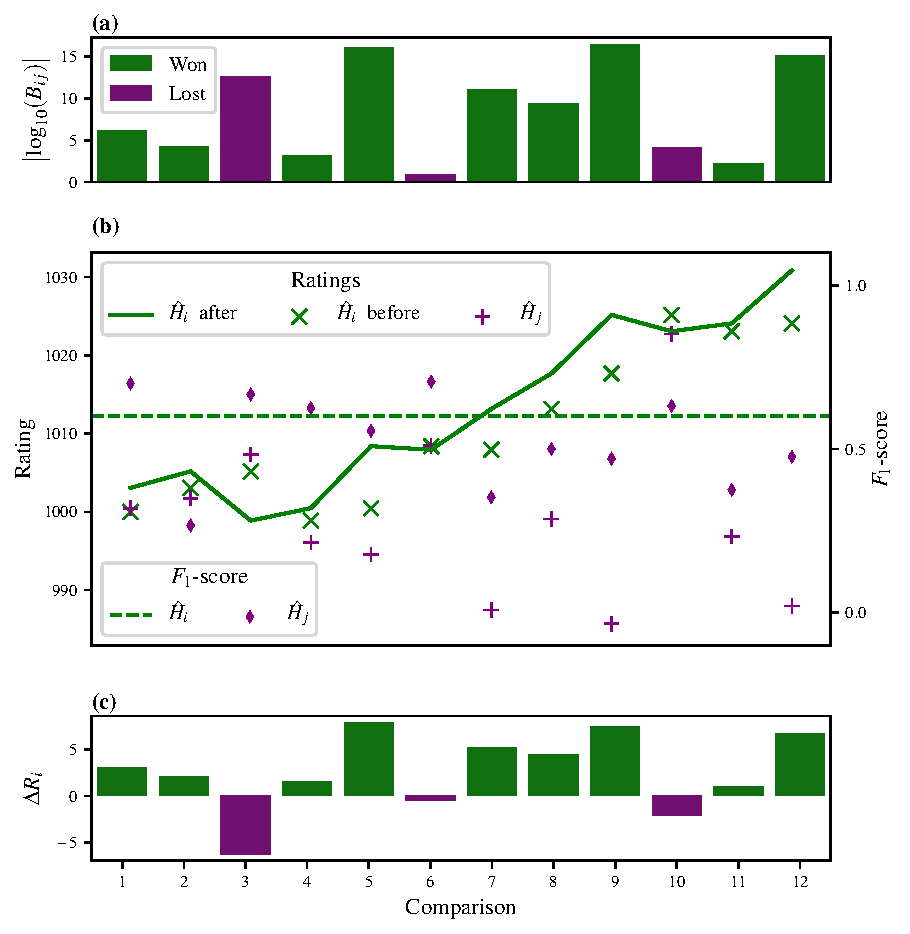
\includegraphics{theoretical_study/figures/single_generation_ratings_progression.pdf}
    \end{center}
    \caption[Single model within a single generation of QMLA genetic algorithm]{
        Progression of \glsentrylong{bfeer}  for a single candidate, $\hi$, within a single generation.
        \textbf{a}, The \glspl{bf} between $\hi$ and some opponents, $\{\hj\}$, 
            from the perspective where $\hi$ \emph{wins} given $\bij > 1 \Rightarrow \log_{10}\bij > 0$, 
            and \emph{loses} otherwise. 
        \textbf{b}, $\hi$'s rating is shown (solid green line) changing according to the \glspl{bf} 
            comparisons with 12 other models from the same generation. 
            Before each comparison, $\hi$'s rating is shown (green cross)
            as well as the rating of its opponent, $\hj$ (purple plus).
            The $F_1$-scores are also shown for $\hi$ (dashed green line) and $\hj$ (purple diamond).
        \textbf{c}, The corresponding change in $\hi$'s rating, $\Delta R_i$. 
        \figtableref
    }
    \label{fig:single_models_elo_ratings}
\end{figure}

Recall that \gls{bfeer} are mediated through random graphs: 
    given $N_m$ models on $\mu$, a given model $\hi$ undergoes some 
    $N_i^{BF} < N_m$ \gls{bf} comparisons. 
In \cref{fig:single_models_elo_ratings} we show the \gls{bf} results 
    and effects on the rating of a random model, $\hi$, where $N_m=60$ and $N_i^{BF}=12$,
    i.e. $\hi$ is directly compared against $20\%$ of contemporary models on $\mu$. 
We see that $\hi$'s rating is effected by whether it wins a given comparison, 
    but also by the strength of evidence provided by the comparison (the \gls{bf}), 
    and the quality of its opposition $\hj$, i.e. the initial rating of $\hj$.
For example, the sixth comparison finds $\hj$ as the superior model, 
    but the evidence is relatively weak and $\hi, \hj$ began with similar ratings, 
    so $R_i$ is not effected drastically. 


\par 
\begin{figure}
    \begin{center}
        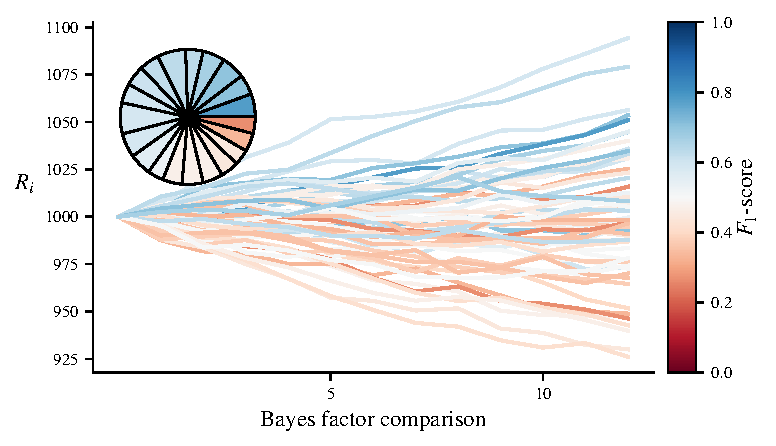
\includegraphics{theoretical_study/figures/single_generation_all_ratings.pdf}
    \end{center}
    \caption[Ratings of all models in a single genetic algorithm generation]{
        Ratings of all $N_m=60$ models in a single \glsentrylong{ga} generation.
        Each line represents a unique model and is coloured by the $\fs$ of that model. 
        \textbf{Inset}, the selection probabilities resulting from the final ratings of this generation. 
        Only $tau=\nicefrac{1}{3}$ of models are assigned selection probability, 
            while the remaining poorer-performing models are discarded. 
        \figtableref
    }
    % TODO replace left of figure with version where elite models are reset to initial rating
    \label{fig:single_generation_all_ratings}
\end{figure}

We extend the single model analysis of \cref{fig:single_models_elo_ratings} to all $N_m$ models 
    in the first generation in \cref{fig:single_generation_all_ratings}.
The general trend is that models of higher $\fs$ have their ratings increased, 
    at the expense of models of lower $\fs$. 
After assessing models thus, the set of models is truncated with rate $\tau=\nicefrac{1}{3}$ to retain only 
    the strongest $20$ candidates,
    which are assigned selection probability, i.e. their chance of being chosen to become a parent during roulette selection, 
    as in \cref{sec:reproduction}.
$N_m$ models are required to populate the next generation:
    the two models with highest $R_i$ -- the \emph{elite} models -- are automatically granted a position;
    the remaining positions are filled through the crossover procedure outlined above.

\par 
\begin{figure}
    \begin{center}
        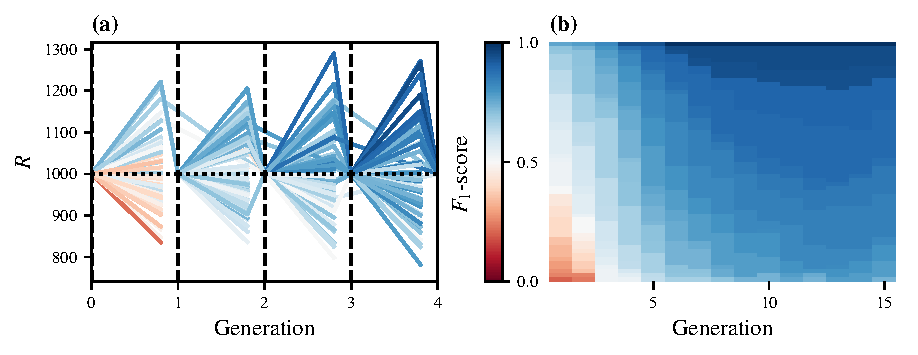
\includegraphics{theoretical_study/figures/gen_alg_instance_combined.pdf}
    \end{center}
    \caption[Instance of QMLA genetic algorithm]{
        A single \gls{instance} of the \gls{qmla} \glsentrylong{}{ga}.
        \textbf{a}, Ratings of all models for the first four generations. 
        Each line in each generation represents a model by its $\fs$. 
        Horizontal dotted lines show the starting rating at that generation. 
        \textbf{b}, Gene pool progression for $N_m=60, N_g=15$. 
        Each tile at each generation represents a model by its $\fs$. 
        \figtableref
    }
    \label{fig:ga_instance}
\end{figure}

We can likewise consider the quality and ratings of models across generations.
In \cref{fig:ga_instance}\textbf{(a)} we see the ratings for models over the first 
    four generations of a \gls{qmla} \gls{instance}:
    the trend suggested by \cref{fig:single_generation_all_ratings} continues,
    where models of higher $\fs$ tend to achieve higher \gls{bfeer}.
The gene pool as a whole tends towards a homogeneous set of high-quality models:
    the final generation consists only of models with $f \geq 0.85$, \cref{fig:ga_instance}\textbf{(b)}. 
Consequently, even in \glspl{instance} where the precise model, $\ho$, is not identified, the \gls{champion model}
    is highly informative, in that it captures many of the same interactions, 
    therefore most-likely providing meaningul insight on the system's physics. 

\par 
\begin{figure}
    \begin{center}
        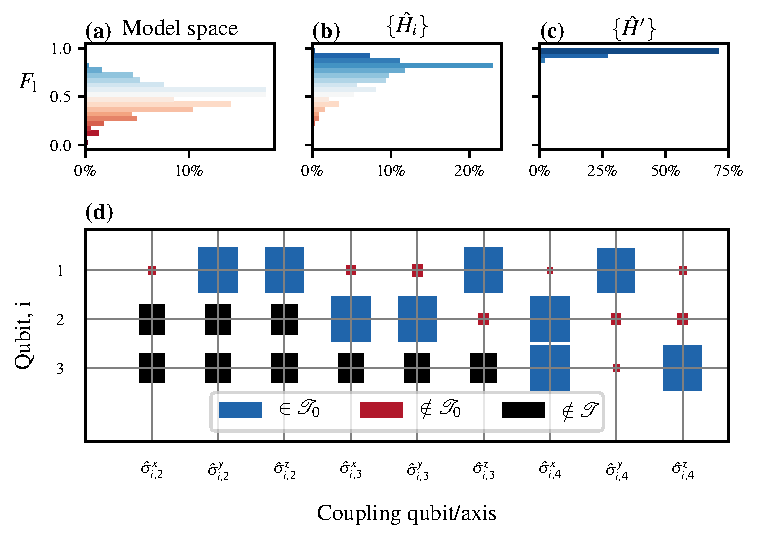
\includegraphics{theoretical_study/figures/gen_alg_run.pdf}
    \end{center}
    \caption[Run of QMLA genetic algorithm]{
        A \gls{run} of the \gls{qmla} \glsentryfull{ga}, consisting of 100 independent \glspl{instance}.
        \textbf{(a)}, The \gls{model space} contains $2^{18}\approx250,000$ candidate models, 
            normally distributed around $f=0.5 \pm 0.14$. 
        \textbf{(b)}, The models explored during the model search of all \glspl{instance} combined, $\{\hat{H}_i\}$.
            \gls{qmla} generates $\sim~43,000$ chromosomes in total across the 100 instances,
                i.e. each \gls{instance} trains $\sim~430$ distinct models;
                Models generated by \gls{qmla} are described overall by a distribution of $f = 0.76 \pm 0.15$, 
        \textbf{(c)}, Champion models from each instance, showing in general \gls{qmla} nominates cahmpion models with
            $f \geq 0.88$ in all instances, 
            and in particular finds the \gls{true model} $\ho$ (with $f=1$) in $72\%$. 
        \textbf{(d)}, Hinton diagram showing the rate at which each term is found in the winning model. 
            The size of the blocks show the frequency with which they are found, while the colour indicates 
            whether that term was (not) in the \gls{true model} in blue (red).
            Terms represetn couplings between two qubits, e.g $\s_{(1, 3)}^{x}$ 
                couples the first and third qubits along the $x$-axis. 
            Available terms involve four qubits with full connectivity, resulting in 18 unique terms 
            (terms with black rectangles are not considered by the \gls{ga}).
        \figtableref
    }
    \label{fig:ga_run}
\end{figure}

Finally, to understand the performance of the \gls{qmla} algorithm overall, 
    we combine 100 independent \glspl{instance} in a \gls{run}, \cref{fig:ga_run}. 
We see that, while the overall \gls{model space} can be characterised by a distribution 
    of models with $\bar{f} = 0.5 \pm 0.14$ (\cref{fig:ga_run}\textbf{(a)}), 
    \gls{qmla} quickly moves to the subspace of high-quality models, 
    i.e. the models explored have median $f = 0.76 \pm 0.15$ (\cref{fig:ga_run}\textbf{(b)}).
This exploration is based on $430 \pm 45$ chromosomes per instance, 
    i.e. \gls{qmla} trains only $0.16\%$ of the $2^{18}$ permitted models. 
Ultimately \gls{qmla} nominates \glspl{champion model} $\{ \hp \}$ with $f \geq 0.88$ in all instances, 
    and precisely identifies $\hp=\ho$ in $72\%$ of instances, \cref{fig:ga_run}\textbf{(c)}. 
Considering the big picture 
    -- where the remit of \gls{qmla} is to identify the interactions \gls{q} undergoes -- 
    we show the rate at which each individual term/gene is included in $\hp$ in 
    \cref{fig:ga_run}\textbf{(d)}. 
Crucially, we see that terms which really are within the true Hamiltonian, $\hat{t} \in \termset_0$, 
    are found at a higher rate than those without, $\hat{t} \notin \termset_0$. 
This level of analysis can be used to post-validate the outcome of \gls{qmla}, 
    i.e. rather than relying on $\hp$ from a single instance, 
    trusting the terms' individual frequencies as evidence that they are of importance when describing 
    the system of interest. 
\par 

\subsection{Device calibration}
The use-case presented in this chapter is restrictive,
    so cannot be considered as a solution to characterising any black box quantum system.
Firstly, the set of conceivable terms must be prescribed in advance to facilitate a chromosome mapping;
    this either limits the range of insight \gls{qmla} can achieve to interactions envisaged by the user,
    or requires a vast set of permissible terms, leading to substantially longer model search phases than shown here. 
Secondly, models were trained using \gls{iqle} in order to learn effectively with relatively few resources. 
\gls{iqle} is only available to train models where we can reliably reverse the evolution of the target system 
    (see \cref{sec:iqle}), and as such it is only useful when we have complete control over \gls{q}, 
    for example where \gls{q} is some quantum simulator. 
\par 
The adaptive \gls{ges} presented in this chapter may therefore prove a useful 
    application of \gls{qmla} in the domain of device calibration,
    in particular to characterise some untrusted quantum simulator.
That is, by using the simulator to implement some target $\ho$, 
    \gls{qmla} can identify which operator is \emph{actually} implemented.
For instance, implementation of a four--qubit model
    relies on high-fidelity two-qubit gates between arbitrary qubit pairs.
\gls{qmla} can effectively reconstruct which operations were and were not faithfully computed,
    i.e. determine in which operations the device failed to perform the intended calculations,
    allowing for the calibration of said device. 
The extension of \gls{qmla} to the characterisation of real quantum devices is one of the main 
    recommendations for future research in the scope of the \gls{qmla} framework beyond this thesis.  